\documentclass{beamer}
\DeclareFontShape{OT1}{cmss}{b}{n}{<->ssub * cmss/bx/n}{} 
\usetheme{default}
\usepackage{amsmath}
\usepackage{amsfonts}
\usepackage{mathbbol}
\usepackage{xcolor} % before tikz or tkz-euclide if necessary
\usepackage{tkz-euclide} % no need to load TikZ
\usepackage{multirow}
\usepackage{lmodern}
\usepackage{bm}

\title{Statistical Machine Learning\\ Part 5}
\author{Horacio G\'omez-Acevedo\\ Department of Biomedical Informatics}
\begin{document}
	\begin{frame}[plain]
		\maketitle
	\end{frame}
\begin{frame}{Probability refresher}
	
	{\bf Formal definition. } A probability space is a triplet $(A, \mathfrak{A},P )$, where $A$ is a (non-empty) set, $\mathfrak{A}$ contains subsets of $A$ called {\it events} (those events form a $\sigma$-algebra of $A$) and a function $P\colon \mathfrak{A}\to [0,1]$ (the so-called {\it probability function}).
	
	{\bf Example.}
	Let's consider the experiment of rolling a die. $A$ will be the outcomes $A=\{ 1,2, \ldots, 6\}$ and $\mathfrak{A}$ will be the subsets of $A$. For instance, the event $E$ consisting of the even number output is $\{2,4,6\}$. The probability function will be defined as 
	\begin{equation*}
		P(E) = \frac{ \textrm{number of elements of }E}{\textrm{number of elements in }A}= \frac{3}{6}
	\end{equation*}
	
\end{frame}

\begin{frame}{Complete system of events}
	We called a {\it complete system of events} a collection  $\{ A_\alpha \}_{\alpha \in I}$ that satisfy:
	\begin{itemize}
		\item $A_\alpha \cap A_\beta = \emptyset$
		\item $\cup_{\alpha \in I} A_\alpha= A$.
	\end{itemize}
 A jigsaw puzzle is a simple visualization of this. $A$ is the whole rectangle and each piece is one of the $A_\alpha$. 
 \begin{figure}[h]
 	\centering
 	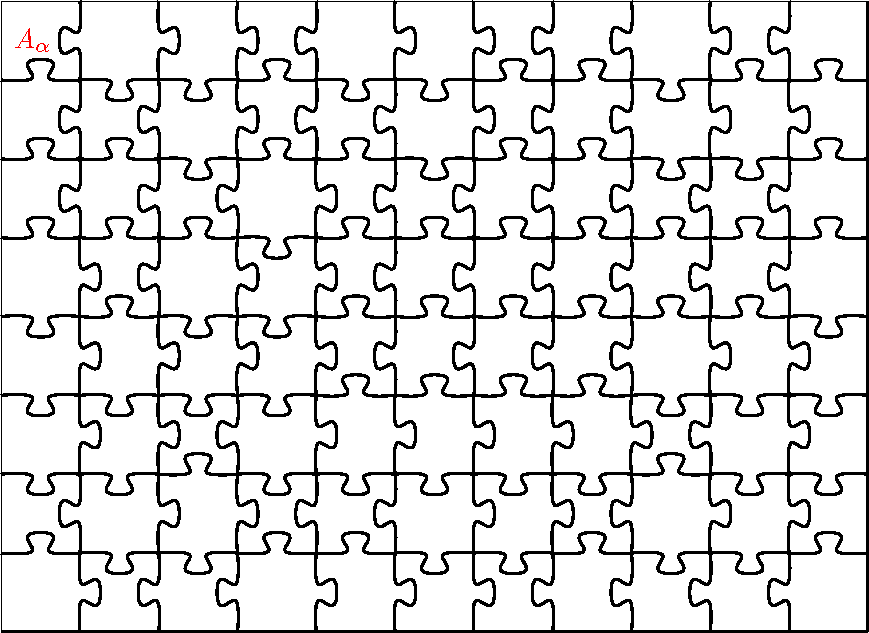
\includegraphics[scale=0.35]{../../Figures/fig_jigsaw.png}
 \end{figure}
\end{frame}

\begin{frame}{Conditional Probabilities}
	If $B$ and $C$ are events and $P(C)>0$, we say that the probability that the event $B$ has occurred given that $C$ has occurred is given by 
	\begin{equation*}
		P(B|C) = \frac{P(B\cap C)}{P(C)}		
	\end{equation*}	

{\bf Total Probability Theorem}. 
If we have a complete system of events $\{A_\alpha\}_\alpha\in I$ with $P(A_\alpha)>0$ for each $\alpha \in I$, then for an arbitrary event $E$ it holds
\begin{equation*}
	P(E) = \sum_{\alpha} P(E|A_\alpha)P(A_\alpha)
\end{equation*}
It is clear that every term $P(E|A_\alpha)P(A_\alpha)=P(A_\alpha \cap E)$. Thus, the probability of $E$ is the sum of every part of $E$ in each $A_\alpha$.
\end{frame}
\begin{frame}{Total Probability Theorem}
Suppose our space is again the jigsaw puzzle rectangle and each piece is $A_\alpha$ as before. The probability measure will be the area cover by an event. In this case our "event" represents the blue letters. Visually the probability of the whole event will be the sum of the blue area in each of the pieces, thus the name "total probability"

 \begin{figure}[h]
	\centering
	
\includegraphics[scale=0.5]{../../Figures/fig_ml_is_fun.png}
\end{figure}

\end{frame}

\begin{frame}{Bayes Theorem}
	Following the same framework as before, we have one of the most useful results in probability
	
	{\bf Bayes theorem.} If $E$ is an event with $P(E)>0$, then
	\begin{equation}
		P(A_\beta |E )= \frac{P(E|A_\beta)P(A_\beta)}{\sum_{\alpha\in I}^{}P(E|A_\alpha)P(A_\alpha)}
		\label{eq:bayes}
	\end{equation}
Note that the numerator of (\ref{eq:bayes}) is $P(E \cap A_\beta)$ whereas the denominator is $P(E)$ according to the total probability theorem!
\end{frame}

\begin{frame}{Bayesian Perspective}
	Unlike the traditional (frequentist) inference, the Bayesian approach tries to determine conclusions about a parameter $\theta$ or unobserved data $\overline{y}$ as probability statements.  For example, given the observed data $y$,  Bayesian statements are based on the conditionals such as  $P(\overline{y}|y)$ for {\it new data} $\overline{y}$, or $P(\theta|y)$ for a parameter $\theta$. So following our Bayes theorem,
	
	\begin{equation}
		{\color{blue}P(\theta| y)}=\frac{{\color{red} P(\theta)} {\color{green}P(y|\theta)}}{\color{green}P(y)}
		\label{eq:bayes2}
	\end{equation}
where $P(y)= \sum_{\theta} P(\theta) P(y|\theta)$ (or in the continuous case $P(y)= \int P(\theta) P(y|\theta) d\theta$). 

The expression  $\color{red} P(\theta)$ is called the {\bf prior}, whereas  $\color{blue} P(\theta|y)$  is called {\bf posterior}, and $\color{green}P(y|\theta)/P(y)$ is called {\bf likelihood}. 

Note that in (\ref{eq:bayes2}) the denominator does not depend on $\theta$.  So, the unnormalized posterior 

\begin{equation*}
	P(\theta|y) \propto P(\theta) \cdot P(y|\theta)
\end{equation*}

 
\end{frame}

\begin{frame}{Density functions}
	When we have a continuous random variable $X$, the probability is calculated by integrals instead of sums. The {\bf probability density function} $f(x)$ describes the probability of an event. 
	
	For instance, let's suppose we have a random variable $X$ distributed as a $N(0,1)$. The density function in this case is defined as
	\begin{equation*}
		f(x)= \frac{1}{\sqrt{2\pi}} \exp(-x^2/2)
	\end{equation*}
Then, the probability that our random variable lies in the interval  $[a,b]$ is given by
\begin{equation*}
		P(a \le X \le b)= \int_a^b f(x)dx = \int_a^b  \frac{1}{\sqrt{2\pi}} \exp(-x^2/2) dx
\end{equation*}
 \begin{figure}[h]
	\centering
	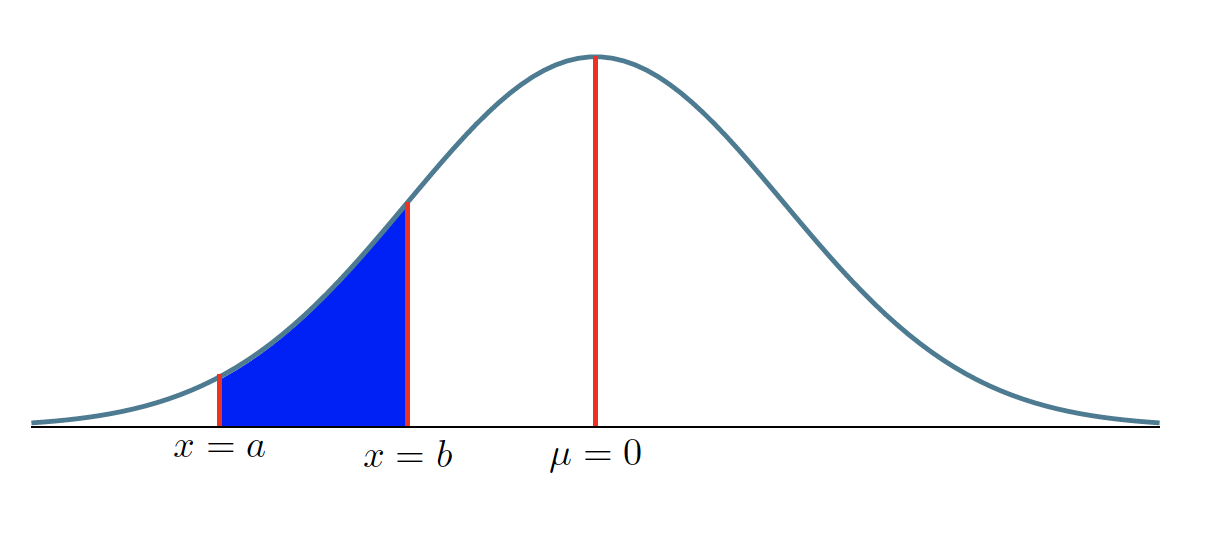
\includegraphics[scale=0.3]{../../Figures/fig_density.png}
\end{figure}

\end{frame}

\begin{frame}{Linear Discriminant Analysis}
	We need to classify an observation into one of $K$ distinct classes ($K\ge 2$). The response variable $Y$ can take on $K$ possibilities. Let $\pi_k$ denote the {\it prior} probability that a randomly chose observation comes from the $k$th class. Let $f_k(X)= P(X=x|Y=k)$ denote the {\it density function} of $X$ for an observation that comes from the $k$th class. We know by the Bayes' theorem
	\begin{equation}
		P(Y=k| X=x)= \frac{\pi_k f_k(x)}{\sum_{i=1}^K \pi_i f_i(x)}
		\label{eq:lda1}
	\end{equation}
 	Let's simplify  {\it posterior probability} , so $p_k(X)=P(Y=k|X)$ 
	
	What have we achieved thus far?
	\begin{itemize}
		\item We have a classifier based on posterior probabilities (\ref{eq:lda1}) by selecting the class with the highest probability. 
		\item The prior information can easily be achieved
		\item The terms $f_k$ are hard to calculate.
	\end{itemize}
\end{frame}


\begin{frame}{Linear Discriminant Analysis $p=1$}
	Let's consider the case that we have $K$ classes and all our observations are in the real line $\mathbb{R}$.
	
	\noindent {\bf Case 1. $f_k(x)$ are normal densities with common variance $\sigma^2$.}
	
	In this case
	\begin{equation*}
		f_k(x)= \frac{1}{\sqrt{2\pi}\sigma} \exp\left( 
		-\frac{1}{2\sigma^2} (x-\mu_k)^2,
		\right)
	\end{equation*}
	where $\mu_k$ are the (estimates) of the mean for each class. Note that the priors $\pi_k$ are estimated based on the proportion of samples in class $k$ from the training set. Thus,
	
	\begin{equation*}
		p_k(x) = \frac{\pi_k \frac{1}{\sqrt{2\pi}\sigma} \exp\left( 
			-\frac{1}{2\sigma^2} (x-\mu_k)^2
			\right)}{\sum_{i=1}^K \frac{1}{\sqrt{2\pi}\sigma} \exp\left( 
			-\frac{1}{2\sigma^2} (x-\mu_i)^2
			\right)}
	\end{equation*}
	The classification rule for $X=x$ states that we will select the class with the largest posterior probability.
	
	
\end{frame}

\begin{frame}{Discriminant Function for Case 1.}
	It can be shown that 
	\begin{equation}
		\begin{split}
			\textrm{Class of }x=& \textrm{argmax}_k \{p_k(x) \}= \textrm{argmax}_k \delta_k(x)\\
			&=\textrm{argmax}_k x \frac{\mu_k}{\sigma^2}- \frac{\mu_k^2}{2\sigma^2} + \log(\pi_k)
		\end{split}
	\label{eq:discriminant}
		\end{equation}
	where $\mathrm{argmax}$ returns the index of the largest value of $p_k(x)$.
 Thus, the discriminant  (\ref{eq:discriminant}) is linear ($ax+b$) and there are $K-1$ points that split the line into $K$ classes.
 
  \begin{figure}[h]
 	\centering
 	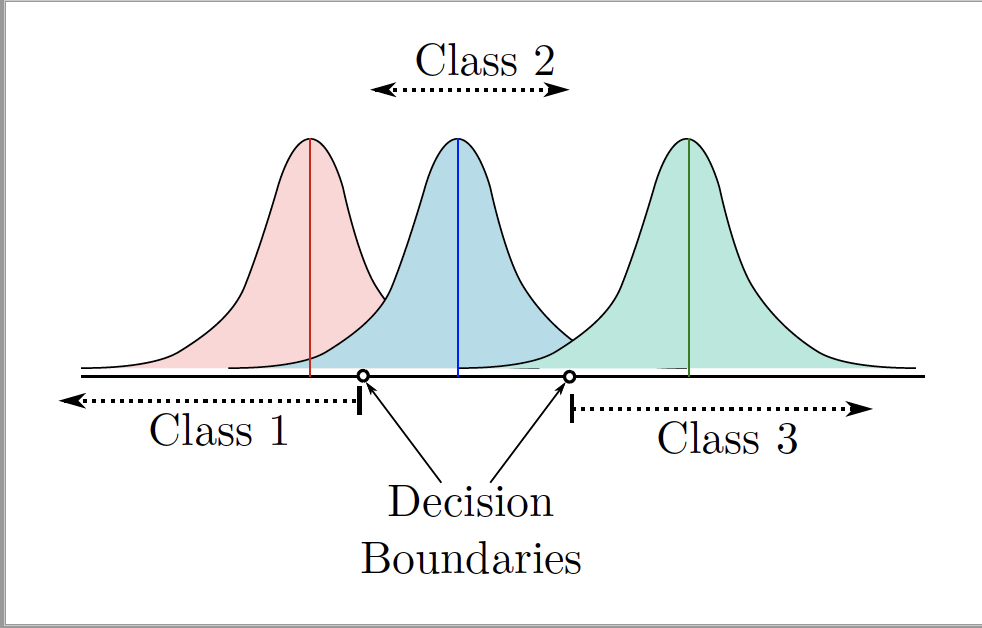
\includegraphics[scale=0.35]{../../Figures/fig_lda.png}
 \end{figure}
\end{frame}

\begin{frame}{Linear Discriminant Analysis (Case 1)}
	Even if we assume that each class has a normal distribution, we need to estimate $\mu_1, \ldots , \mu_K$, $\pi_1,\ldots,\pi_K$ and $\sigma$. 
	
	Formula (\ref{eq:discriminant}) will still be valid if we plug in the following estimates
	\begin{equation*}
		\begin{split}
			\hat{\mu}_k&= \frac{1}{n_K} \sum_{i:y_i  \textrm{ in class }k} x_i\\
		\hat{\sigma}^2 &= \frac{1}{n-K} \sum_{k=1}^{K} \sum_{i:y_i  \textrm{ in class } k}	 (x_i -\hat{\mu}_k)^2\\
		\hat{\pi}_k &= \frac{n_k}{n}
	\end{split}
	\end{equation*}
\end{frame}

\begin{frame}{Linear Discriminant Analysis (Case 2)}
	Once we have found our discriminant function for the case $p=1$, now we will move to higher dimensions ($p\ge 2$).  Let's assume that $\mathbf{X}=(X_1,\ldots, X_p)$ are drawn from a multivariate Gaussian with a class-specific mean vector $E(\bm{X})=\bm{\mu}=(\mu_1,\ldots,\mu_p)$,and a common variance-covariance matrix $\bm\Sigma$. 
	The general multivariate normal density is written as
	\begin{equation}
		f(\bm{x})= \frac{1}{(2 \pi)^{p/2} | \bm{\Sigma} |^{1/2}}\exp\left( - \frac{1}{2} (\bm{x} - \bm{\mu})^T \bm{\Sigma}^{-1} (\bm{x}-\bm{\mu}) \right)
	\end{equation}	
where $|\bm{\Sigma}|$ is represents the determinant of the matrix $\bm{\Sigma}$. So, the LDA for higher dimensions assumes that observations in the $k$th class are drawn from a multivariate distributions $N(\bm{\mu}_k, \bm{\Sigma})$ 

\end{frame}

\begin{frame}{Linear Discriminant Analysis (Case 2)}
	 \begin{figure}[h]
		\centering
		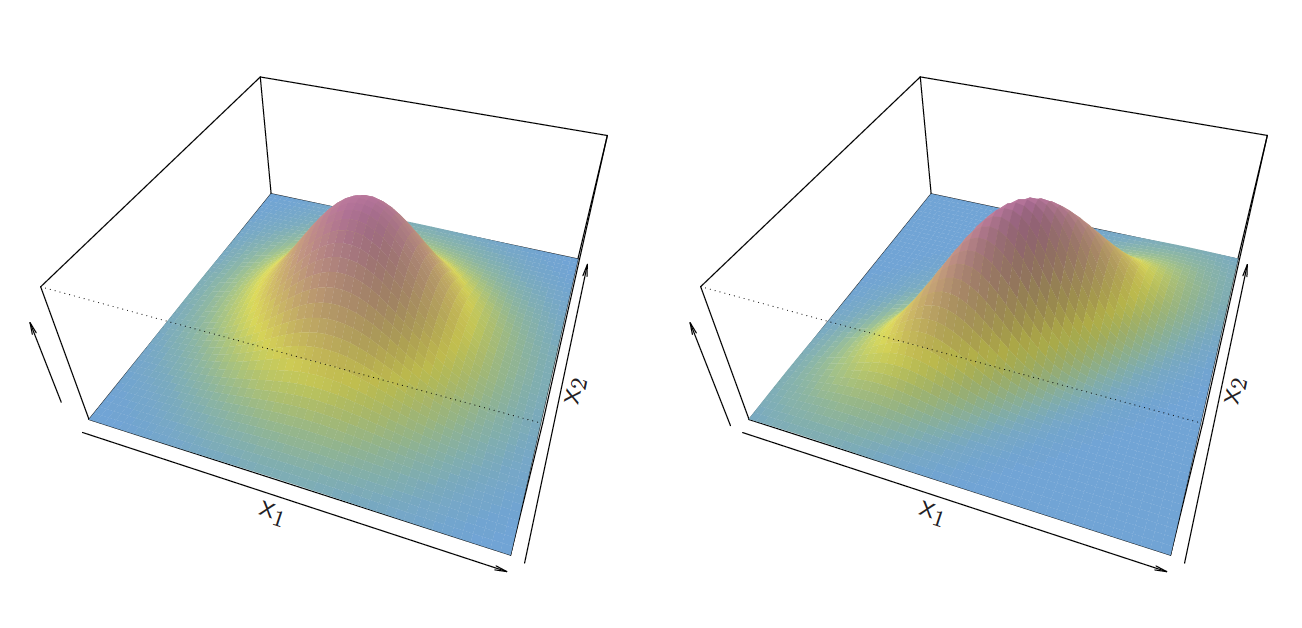
\includegraphics[scale=0.35]{../../Figures/fig_multiv_gauss.png}
	\end{figure}
	
	
	As for the discriminant function for higher dimensions
	
	\begin{equation*}
		\delta_k(\bm{x})= \bm{x}^T \bm{\Sigma}^{-1} \bm{\mu}_k - \frac{1}{2} \bm{\mu}_k^T \bm{\Sigma}^{-1}\bm{\mu}_k + \log(\pi_k)
	\end{equation*}
\end{frame}

\begin{frame}{Linear Discriminant Analysis (Case 2)}
	The Bayes decision boundaries will be calculated by pairs of indexes. Namely, if $\bm{x}$ is in the decision boundary of $k$ and $l$ then
	\begin{equation*}
		\bm{x}^T \bm{\Sigma}^{-1} \bm{\mu}_k - \frac{1}{2} \bm{\mu}_k \bm{\Sigma}^{-1} \bm{\mu}_k= 	\bm{x}^T \bm{\Sigma}^{-1} \bm{\mu}_l - \frac{1}{2} \bm{\mu}_l \bm{\Sigma}^{-1} \bm{\mu}_l
	\end{equation*}
Solving this equation reduces to something like this
\begin{equation*}
	\bm{x}^T \cdot \bm{v}= r
\end{equation*}
Thus, we need to calculate the vector $\bm{v}=(v_1,\ldots,v_p)$ such that 
\begin{equation*}
	v_1 x_1 + \cdots + v_p x_p = r
\end{equation*} 
In $\mathbb{R}^2$ this equation represents a line. 
\end{frame}
\begin{frame}{Linear Discriminant Analysis (Case 2)}
	Thus, when we have multiple classes there will be lines dividing the plane as shown below
	\begin{figure}[h]
		\centering
		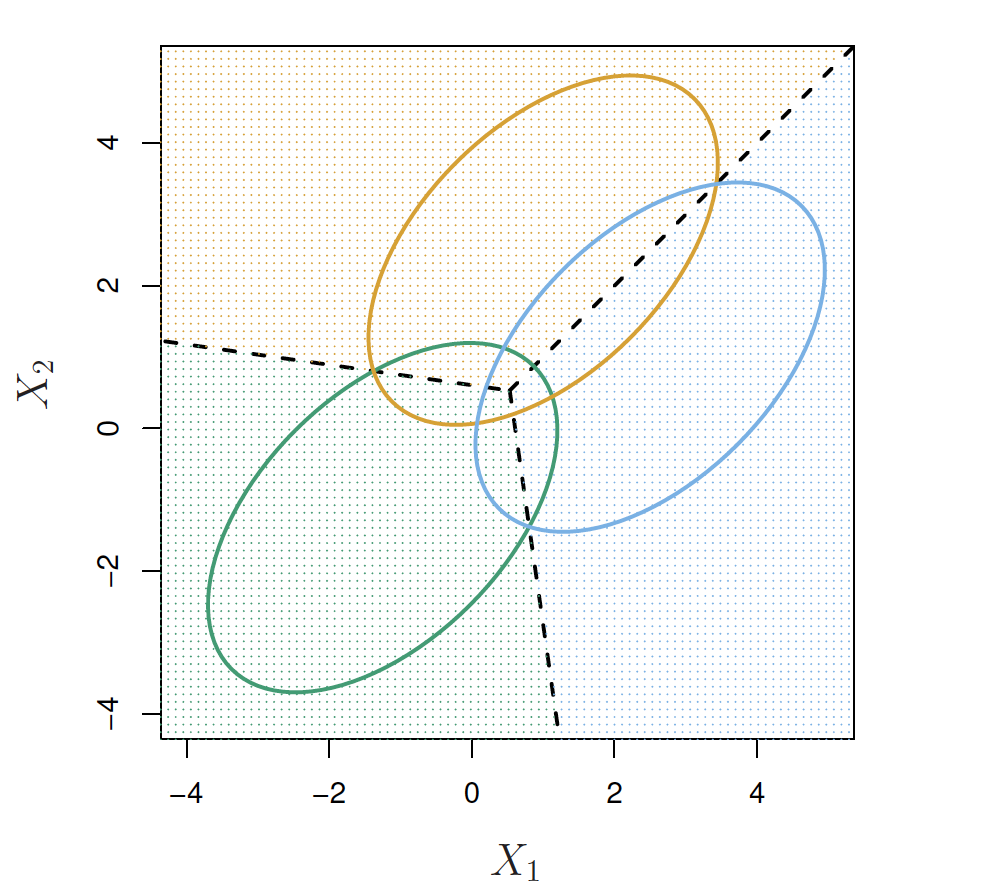
\includegraphics[scale=0.35]{../../Figures/fig_lda_2d.png}
	\end{figure}
	
\end{frame}

\begin{frame}{Linear Discriminant Analysis}
	If we use LDA for binary classification we observe
	\begin{itemize}
		\item LDA has very low classification errors, which is due to the fact that approximates the Bayes classification.
		\item LDA will be off when the confusion matrix is "unbalanced". One remedy for this situation is to lower the threshold of 50\% in the classifier to say 25\%. 
	\end{itemize}
\end{frame}

\begin{frame}{References}
	
	Materials and some of the pictures are from (1),(2), and (3).
	\begin{enumerate}
		\item Gareth James et al. {\it An Introduction to Statistical Learning with applications in R}. Springer (2015)
		\item Richard O. Duda et al. {\it Pattern Classification} John Wiley (2001). 
		\item Aur\'elien G\'eron. {\it Hands-on Machine Learning with Scikit-Learn \& TensorFlow} O'Relly (2017)
		\item Wiebe R. Pestman {\it Mathematical Statistics} de Gruyter (1998)
	\end{enumerate}	
	
	I have used some of the graphs by hacking TiKz code from StakExchange, Inkscape for more aesthetic plots and other old tricks of \TeX
\end{frame}	

\end{document}